% Requires: \usepackage{pgfplots}
% Generated by benchmark/memorisation.py -- do not edit by hand.
\begin{figure}[t]
\centering
\definecolor{fpblue}{HTML}{2A78D6}
\definecolor{fporange}{HTML}{EB6834}
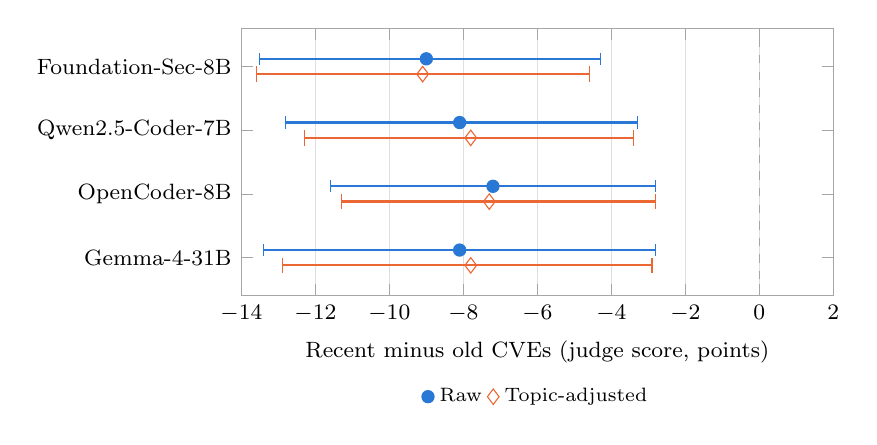
\begin{tikzpicture}
\begin{axis}[
  scale only axis, width=0.62\columnwidth, height=3.4cm,
  xmin=-14, xmax=2, ymin=0.4, ymax=4.6,
  ytick={4,3,2,1}, yticklabels={Foundation-Sec-8B,Qwen2.5-Coder-7B,OpenCoder-8B,Gemma-4-31B},
  y tick label style={font=\footnotesize}, x tick label style={font=\footnotesize},
  xlabel={\footnotesize Recent minus old CVEs (judge score, points)},
  xmajorgrids, grid style={gray!25}, axis line style={gray!70}, tick style={gray!70},
  legend style={font=\scriptsize, at={(0.5,-0.30)}, anchor=north, draw=none}, legend columns=2,
  legend cell align=left,
]
\addplot[gray!70, dashed, forget plot] coordinates {(0,0.4) (0,4.6)};
\addplot[only marks, mark=*, mark size=2.2pt, color=fpblue,
         error bars/.cd, x dir=both, x explicit, error bar style={line width=0.8pt}]
  coordinates {(-9.0,4.12) -= (4.5,0) += (4.7,0) (-8.1,3.12) -= (4.7,0) += (4.8,0) (-7.2,2.12) -= (4.4,0) += (4.4,0) (-8.1,1.12) -= (5.3,0) += (5.3,0)};
\addlegendentry{Raw}
\addplot[only marks, mark=diamond, mark size=2.8pt, color=fporange, mark options={fill=white},
         error bars/.cd, x dir=both, x explicit, error bar style={line width=0.8pt}]
  coordinates {(-9.1,3.88) -= (4.5,0) += (4.5,0) (-7.8,2.88) -= (4.5,0) += (4.4,0) (-7.3,1.88) -= (4.0,0) += (4.5,0) (-7.8,0.88) -= (5.1,0) += (4.9,0)};
\addlegendentry{Topic-adjusted}
\end{axis}
\end{tikzpicture}
\caption{Judge score on recent CVEs (2022--2024, 325 records) minus old CVEs ($\leq$2015,
357 records), CVEfixes test records only. Bars are 95\% bootstrap intervals over records; the
topic-adjusted estimate compares the two groups within each question topic. Values below zero mean a model
does worse on recent vulnerabilities.}
\label{fig:memorisation}
\end{figure}
